\documentclass[xcolor=table]{beamer}

\usepackage{lscape, amsmath, amsfonts, amssymb, setspace, theorem, wrapfig, graphicx, float, multirow, subfig, color, rotating, multicol, datetime, natbib, venndiagram, pstricks, xkeyval, tikz, etoolbox, url, hyperref, nth}

\usepackage[T1]{fontenc}
\usepackage[latin1]{inputenc}
\usepackage[english]{babel}

\title{GV217 - Conflict Analysis}
\subtitle{University of Essex - Department of Government}
\date{Week 20 -- 14 February, 2020}				% or you can specify a date, just write it down instead of "\today"
\author{Lorenzo Crippa} 

\usetheme[progressbar=frametitle]{metropolis}
\usecolortheme{seahorse}						% try others: wolverine; crane...

\begin{document}
\frame{
\titlepage
}

\begin{frame}{Recap: Greed \emph{vs} Grievance}
\begin{enumerate}
\item What is Greed also referred to as? \pause
\item What are the two elements of this aspect? \pause
\item Can you give an example of how we could operationalize (measure) both?
\end{enumerate}
\end{frame}

\frame{
\frametitle{Rationalist explanations for war}
\begin{itemize}
\item Rationality: Ex-ante expectations and ex-post knowledge \pause
\item War is inefficient ex post \pause
\item \textcolor{red}{Key question: What prevents states from locating a bargain both sides would prefer to a fight?}
\end{itemize}
}

\frame{
\frametitle{Fearon 1995}
Fearon (1995) advances 3 rational explanations to answer the \textcolor{red}{key question}. \pause

\begin{enumerate}
\item Private information and incentives to misrepresent \pause
	\begin{itemize}
	\item[] $\rightarrow$ costly signals \pause
	\end{itemize}
\item Commitment problems \pause
\item Issue indivisibility \pause
\end{enumerate}

All relate to \textbf{bargaining space}
}

\frame{
\frametitle{Incentive to misrepresent: Japan-Russia 1904-1905}
\textbf{Both} Russia and Japan had private information $\rightarrow$ information asymmetry \pause

\begin{itemize}
\item Information asymmetry:
	\begin{itemize}
	\item[--] Unknown to Russia, Japan had used spies to gain more information. \pause It knew with greater certainty its strength \pause
	\item[--] Russia thought that Japan was weak \pause \textbf{but} it had been developing its military capabilities \pause
	\end{itemize}
\item Conflict over Manchuria and Korea. \pause
\item In the build up to the conflict, Russia was making very low offers to Japan, thinking that it was stronger. \pause
\item Even if the Japanese had disclosed their full power, Russia would have been unlikely to believe. Why? \pause because there are incentives to misrepresent $\rightarrow$ war.
\end{itemize}
}

\frame{
\frametitle{Costly signals}
``To be \textbf{genuinely} informative about a state's \textbf{actual} willingness or ability to fight, a signal must be costly in such a way that a state with lesser resolve or capability might not wish to send it.'' (Fearon, 1995:397) \pause

$\rightarrow$ Actions that generate a \textbf{real} risk of war are most informative
}

\frame{
\frametitle{Russia-Ukraine conflict (2014)}
\begin{center}
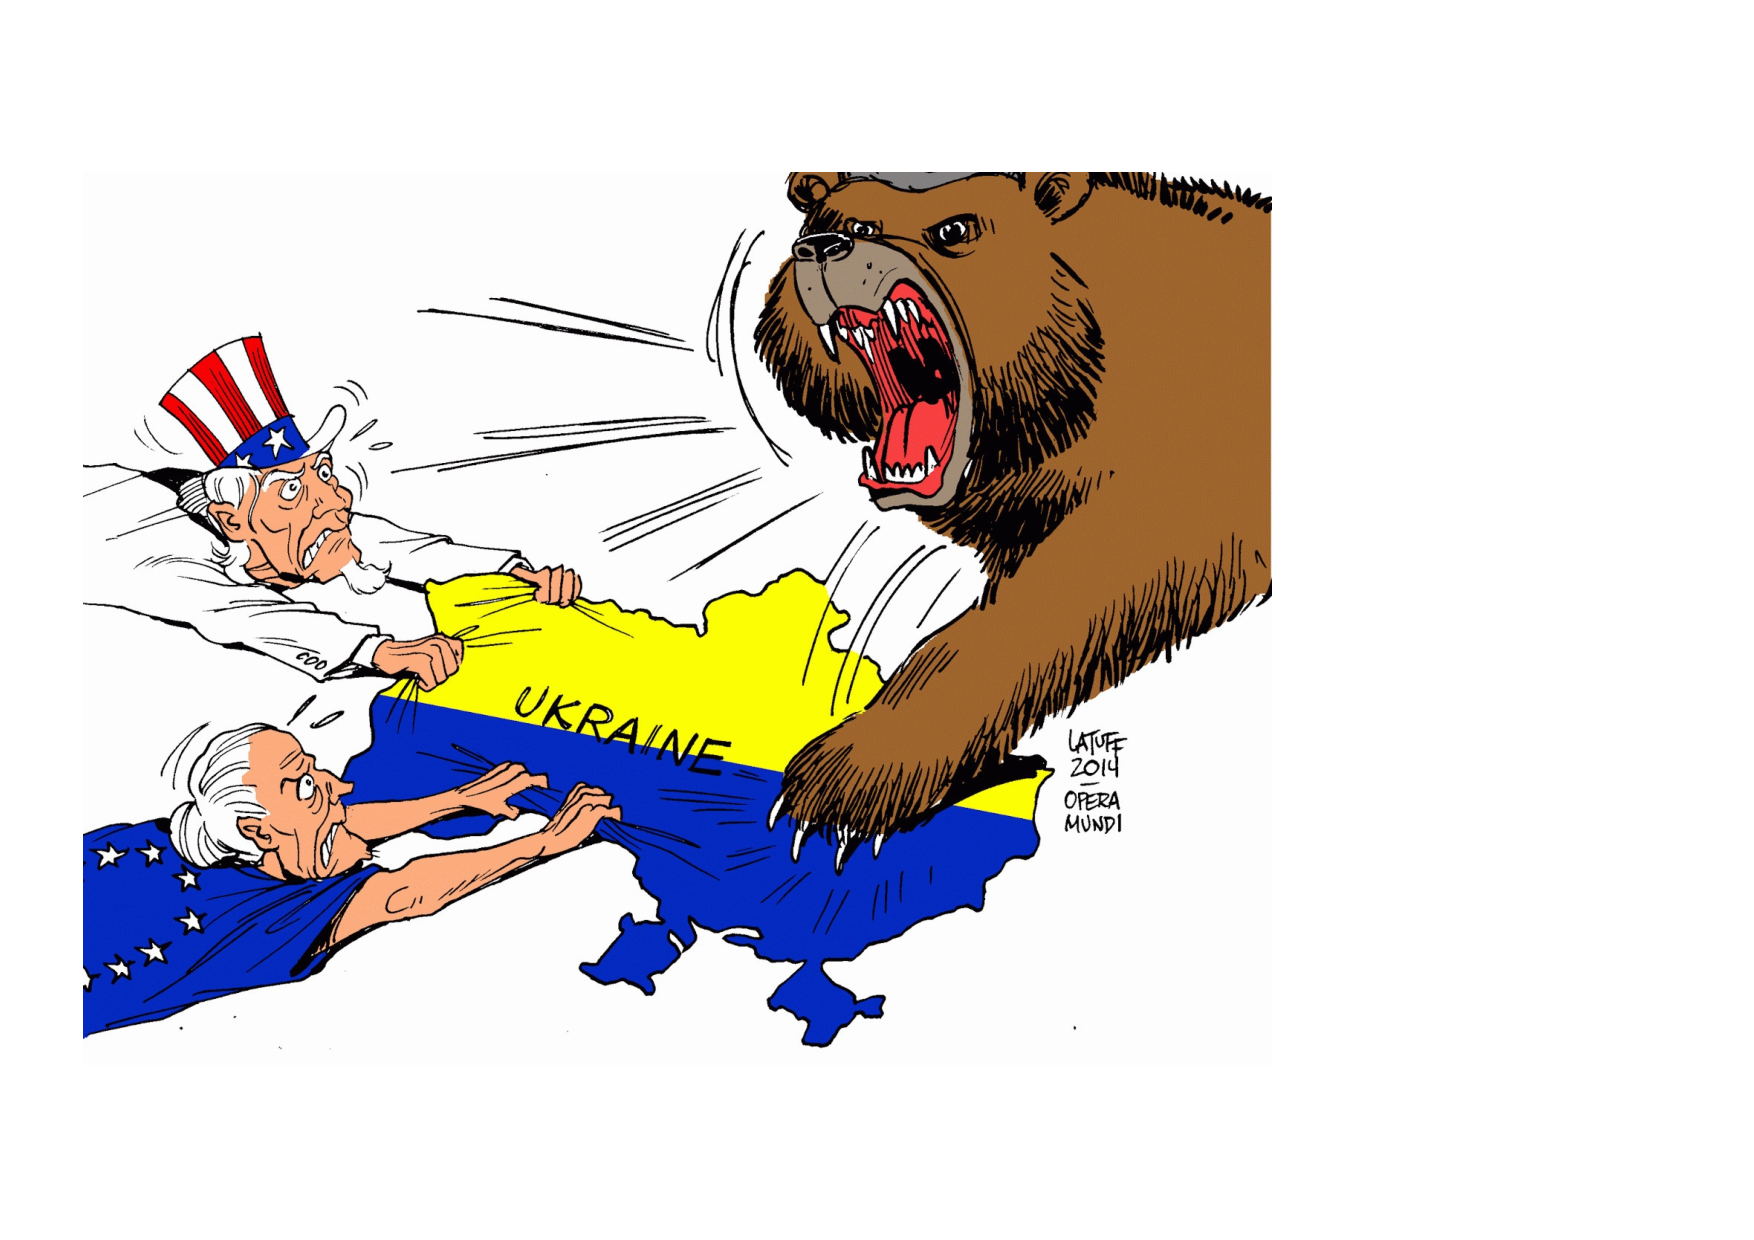
\includegraphics[width=80mm]{pictures/week_20_RU_UA.pdf}
\end{center}

Was Russian invasion of Crimea a costly signal? Why? \pause \\ Yes, arguably: \pause ``EU/NATO stay out of our back yard''. Russia risked war with the West over this territory.
}

\frame{
\frametitle{First Mover Advantage}
Pearl Harbour, 1941

The US fleet was at anchor in Pear Harbour. The Japanese knew that if they struck first, they could severely diminish US capacities in the Pacific. The U.S. did not expect Japan to attack \pause

\textcolor{red}{How does the commitment problem explain this?}
}

\frame{
\frametitle{Preemptive war}
World War I.

Some have argued that the German and Austro-Hungarian empires challenged Russia in the Balkans before WWI because they believed that Russia was a growing power and wished fight now rather than later. Of course, they did not expect France and the UK to become involved. \pause

\textcolor{red}{How does the commitment problem explain this?}
}

\frame{
\frametitle{Final exercise: Peace process in Colombia}
\begin{center}
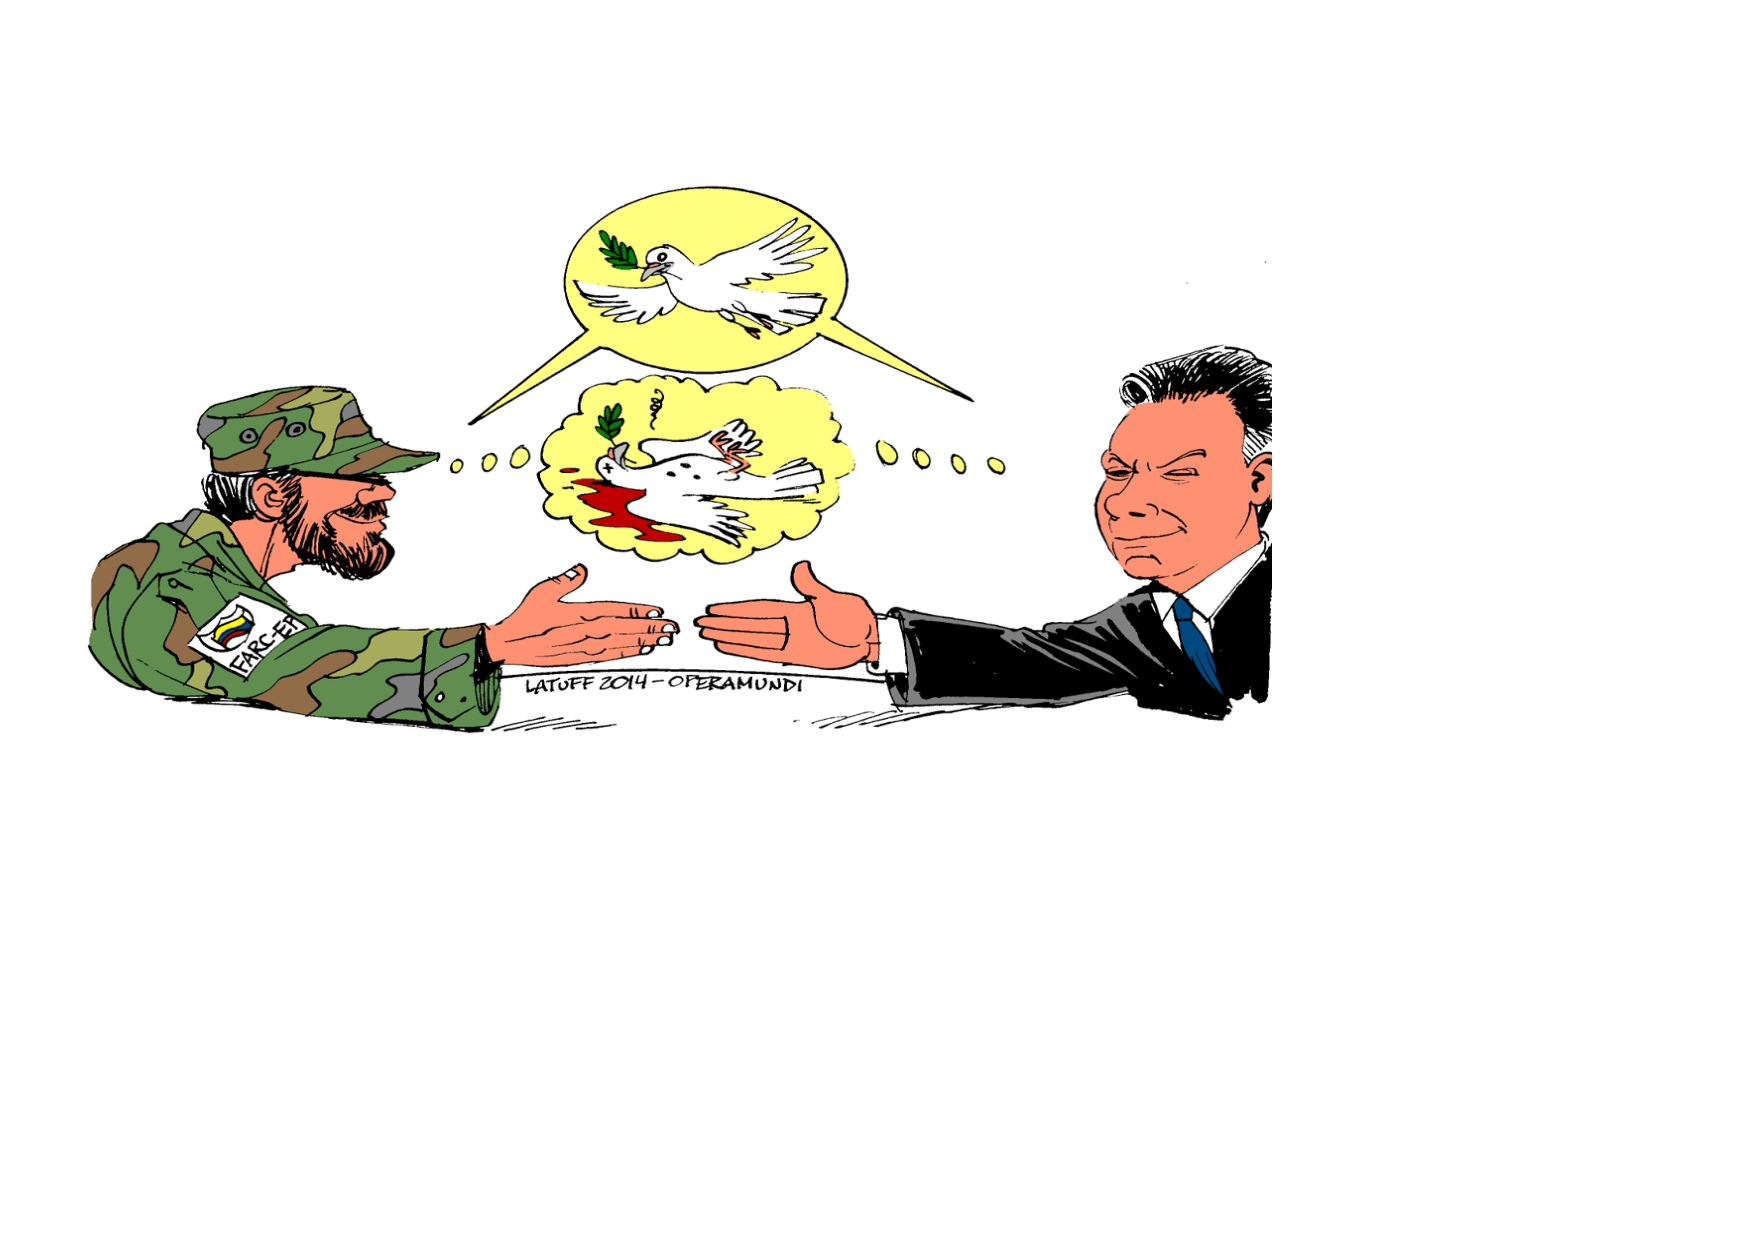
\includegraphics[width=80mm]{pictures/week_20_CO.pdf}
\end{center}

\begin{itemize}
\item Get in groups of 2-3 people
\item Read the assignment and answer the three questions
\item Present your findings to the other groups
\item Do you agree? 
\end{itemize}
}

\frame{
\frametitle{Conclusion}
\begin{center}
All clear? More questions? \\
See you next week!
\end{center}
}


\end{document}
